\section{Erstellen der Doubly-connected Edge List}
\subsection{Graph Klasse}
Die zweidimensionalen Operationen der Anwendung werden von der \icode{Graph}-Klasse durchgeführt. 
Übergibt man dieser eine Liste aus Linien, welche jeweils aus einem Start- und Endortsvektor bestehen, wird auf diesen basierend eine DCEL berechnet.
Dafür werden die drei graphischen Elemente der Typen \icode{Edge}(Kante), \icode{Node}(Knoten) und \icode{Face}(Fläche) gespeichert.

\subsection{Verarbeitung der Linien}
Beginnend werden gleichzeitig die Knoten und Kanten der zu generierenden DCEL erstellt.
\subsection{Vector-to-Node Konvertierung}
Aus einem Ortsvektor kann die Funktion \icode{createNode()} einen kongruenten Knoten mit gleichen Ursprungskoordinaten, aber ohne Referenz auf eine anliegende Kante, erstellen. 
Desweiteren wird, falls ein Knoten zu einem abgefragten Punkt schon generiert wurde, dieser zurückgeben.
\begin{code}[\icode{createNode()} Funktion]
	private Node createNode(Vector p) {
		for (Node n : nodes) {
			if (n.getOrigin().equals(p)) {
				return n;
			}
		}
		nodes.add(new Node(p));
		return (nodes.get(nodes.size() - 1));
	}
\end{code}
\subsection{Line-to-Edge Konvertierung}
\label{subsec:ltoe} 
Die \icode{processData} Funktion greift auf \icode{createNode()} zu und erstellt die Liste aus Kanten mit den jeweiligen Start- und Endknoten.
Auch hier gibt es noch keine abgespeicherten Zusammenhänge zwischen den einzelnen Kanten.
\begin{code}[Line-to-Edge Konvertierung]
private void processData(ArrayList<Line> ls) {
	for (Line l : ls) {
		edges.add(new Edge(createNode(l.getP1()), createNode(l.getP2())));
	}
}
\end{code}
Basierend auf dieser Grundlage müssen alle folgenden Kalkulationen der \icode{Graph}-Klasse durchgeführt werden.
\subsection{Zwillingskantengenerierung}
Durch Vertauschen der Start- und Endknoten wird nun für jede existente Kante eine entgegengesetzt-laufende komplementäre \q{Zwillingskante} gebildet.
In der Anwendung wird so die Liste der Kanten um ihre Größe erweitert.
Direkt nach dem Hinzufügen der Zwillingskante wird jeweils eine Referenz erstellt, welche beide Zwillinge miteinander verknüpft. 
Durch die Zwillingskanten werden folgende Operationen in der DCEL vereinfacht, da jede Fläche nun von einer eindeutigen Menge an Kanten begrenzt ist und ein Umlaufsinn dieser festgestellt werden kann.

\subsection{Nachfolger- und Vorgängerermittlung}
Für die Erstellung der Nachfolger- und Vorgängerreferenzen zwischen den Kanten, werden alle ausgehenden Kanten $E$ eines Knotens $N_i$ betrachtet.
Anschließend sortiert die Anwendung diese mittels der \icode{angle()}-Methode anhand des Winkels.
Dabei wird die jeweilige Kante $E_i$ in einen Vektor, welcher zwischen die beiden Kantenknoten gespannt werden kann, konvertiert, damit die \icode{angle()}-Funktion aufrufbar ist.
Diese gibt den Winkel des Vektors zur x-Achse im Intervall $(-\pi,\pi]$ aus.
Aus den angeordneten Kanten $E$ lassen sich unter Beachtung des mathematisch positivem Umlaufsinnes der Kanten an den Flächen nun folgende Beziehungen ableiten. 
\begin{enumerate}
	\item Die Zwillingskante von $E_{i+1}$ ist der Vorgänger von $E_i$
	\item $E_{i-1}$ ist der Nachfolger der Zwillingskante von $E_i$ 
\end{enumerate}
\begin{Bild}{Veranschaulichung 1. und 2.}
	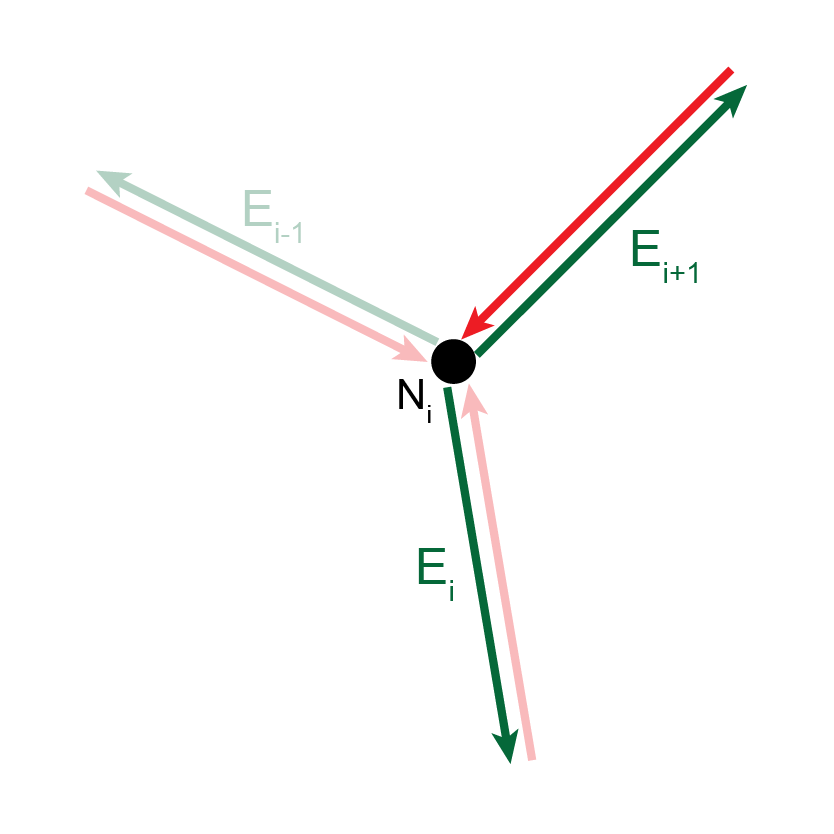
\includegraphics[width = 70mm]{Bilder/Beziehung1Kanten}
		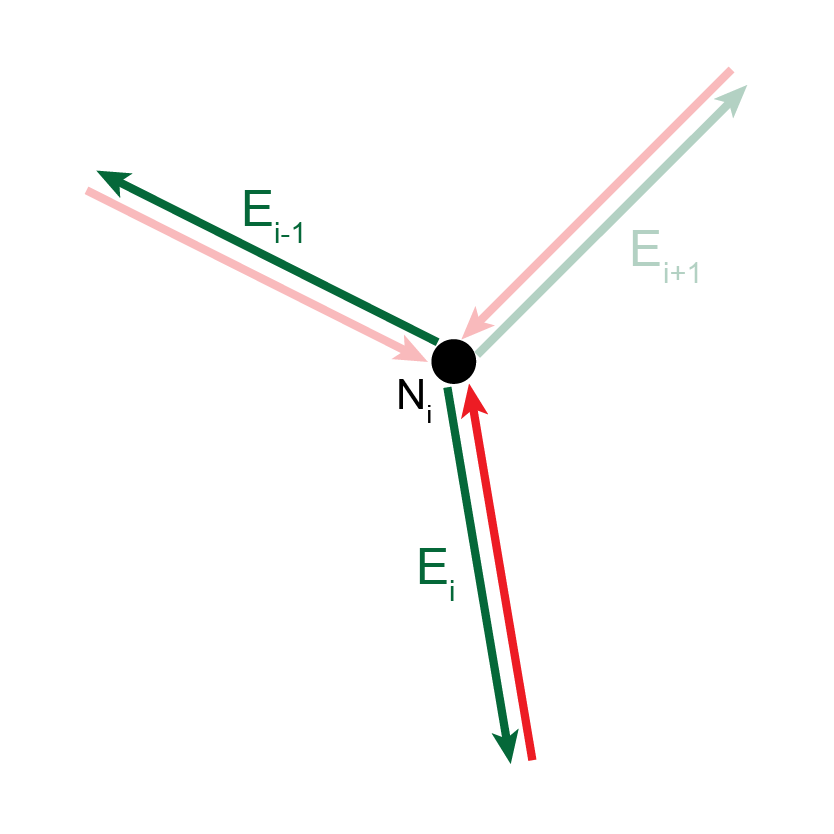
\includegraphics[width = 70mm]{Bilder/Beziehung2Kanten}
\end{Bild}
Falls $i-1$ bzw. $i+1$ die Indices der Menge $E$ mit $n$ Elementen überschreiten, wird anstattdessen $E_n$ bzw. $E_0$ gewählt. \\
Der aufgeführte Algorithmus wird für alle Knoten $N$ der DCEL fortgeführt, sodass alle Referenzen zwischen den Kanten fertiggestellt werden. 
\begin{code}[Zuweisung der Beziehungen im Programm; \icode{nodeEdges} ist eine zweidimensionale ArrayList, die f{\"u}r jeden Knoten eine sortierte ArrayList aus Kanten enth{\"a}lt]
	for (ArrayList<Edge> e : nodeEdges) {
		for (int i = 0; i < e.size(); i++) {
			e.get(i).setPrev(e.get((i + 1) \% e.size()).getTwin());
			e.get(i).getTwin().setNext(e.get(Math.floorMod((i - 1), e.size())));
		}
	}
\end{code}

\subsection{Flächenerstellung}
Durch das Vorliegen der DCEL Kanten können alle Flächen des Graphen erschlossen werden.
Dabei wird bei dem Element $E_0$ der Kantenliste begonnen und solange der Nachfolger über die Verknüpfung ermittelt, bis die Ursprungskante wieder erreicht wurde.
Die ermittelte Fläche $F_0$ besitzt als anliegende Kante so die Kante $E_0$.
Alle in der Fläche enthaltenen Kanten werden bei der fortlaufenden Rechnung ignoriert, sodass die alle anderen Flächen $F$ analog errechnet werden können.
Das äußere Gebiet des planaren Graphen, also in der DCEL der Umriss, kann durch den Drehsinn der Kanten dieser Fläche festgestellt werden, denn dieser ist als einziger mathematisch negativ.
In der Anwendung wird dafür die Gaußsche Trapezformel verwendet, welche bei einem umgekehrten Drehsinn einen negativen Flächeninhalt ausgibt.

\begin{Bild}{Flächenberechnung. Dargestellt: Anliegende Kante(Cyan), Kanten(grün) und Fläche(gelb)}
	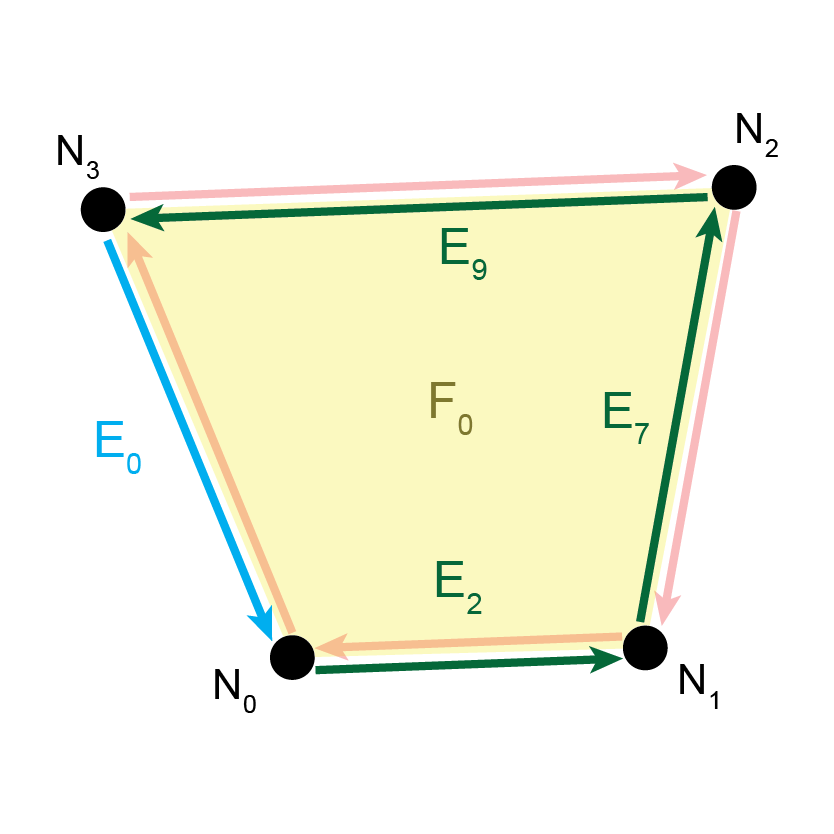
\includegraphics[width = 90mm]{Bilder/FlaecheBerechnung}
\end{Bild}

\subsection{Vervollständigung der Knoten}
Die letzte nötige Referenz ist die einer anliegenden Kante eines Knotens.
Dafür wird für die Knoten $N$ eine Kante ermittelt, die ihren Usrpung in dem jeweiligen Knoten hat.
Die DCEL ist mit diesem Schritt fertiggestellt und bildet die Grundlage für alle folgenden dreidimensionalen Berechnungen.\label{key}
